\documentclass[12pt,fullpage,letterpaper]{article}

\newenvironment{proof}{\noindent{\bf Proof:}}{\qed\bigskip}

\newtheorem{theorem}{Theorem}
\newtheorem{corollary}{Corollary}
\newtheorem{lemma}{Lemma} 
\newtheorem{claim}{Claim}
\newtheorem{fact}{Fact}
\newtheorem{definition}{Definition}
\newtheorem{assumption}{Assumption}
\newtheorem{observation}{Observation}
\newtheorem{example}{Example}
\newcommand{\qed}{\rule{7pt}{7pt}}

\newcommand{\assignment}[4]{
\thispagestyle{plain} 
\newpage
\setcounter{page}{1}
\noindent
\begin{center}
\framebox{ \vbox{ \hbox to 6.28in
{\bf CS446: Machine Learning \hfill #1}
\vspace{4mm}
\hbox to 6.28in
{\hspace{2.5in}\large\mbox{Problem Set #2}}
\vspace{4mm}
\hbox to 6.28in
{{\it Handed Out: #3 \hfill Due: #4}}
}}
\end{center}
}


\newcommand{\handout}[3]{
\thispagestyle{plain} 
\newpage
\setcounter{page}{1}
\noindent
\begin{center}
\framebox{ \vbox{ \hbox to 6.28in
{\bf CS446: Machine Learning \hfill #1}
\vspace{4mm}
\hbox to 6.28in
{\hspace{2.5in}\large\mbox{#2}}
\vspace{4mm}
\hbox to 6.28in
{{\it Handed Out: #3 \hfill Name (NetID): \rule[-2pt]{4cm}{0.1pt} }}
}}
\end{center}
}


\newcommand{\assgsoln}[4]{
\thispagestyle{plain} 
\newpage
\setcounter{page}{1}
\noindent
\begin{center}
\framebox{ \vbox{ \hbox to 6.28in
{\bf CS446: Machine Learning \hfill #1}
\vspace{4mm}
\hbox to 6.28in
{\hspace{2.5in}\large\mbox{Problem Set #2 Solutions}}
\vspace{4mm}
\hbox to 6.28in
{{\it Handed Out: #3 \hfill Handed In: #4}}
}}
\end{center}
}


\newcommand{\solution}[4]{
\thispagestyle{plain} 
\newpage
\setcounter{page}{1}
\noindent
\begin{center}
\framebox{ \vbox{ \hbox to 6.28in
{\bf CS446: Machine Learning \hfill #4}
\vspace{4mm}
\hbox to 6.28in
{\hspace{2.5in}\large\mbox{Problem Set #3}}
\vspace{4mm}
\hbox to 6.28in
{#1 \hfill {\it Handed In: #2}}
}}
\end{center}
\markright{#1}
}


\newenvironment{algorithm}
{\begin{center}
\begin{tabular}{|l|}
\hline
\begin{minipage}{1in}
\begin{tabbing}
\quad\=\qquad\=\qquad\=\qquad\=\qquad\=\qquad\=\qquad\=\kill}
{\end{tabbing}
\end{minipage} \\
\hline
\end{tabular}
\end{center}}

\def\Comment#1{\textsf{\textsl{$\langle\!\langle$#1\/$\rangle\!\rangle$}}}


\usepackage{amsmath}
\usepackage{graphicx}
\usepackage{amsfonts}
\usepackage{amssymb}

\oddsidemargin 0in
\evensidemargin 0in
\textwidth 6.5in
\topmargin -0.5in
\textheight 9.0in

\begin{document}

\solution{Hsiang-Wei Hwang}{\today}{1}{Spring 2017}
% Fill in the above, for example, as follows:
% \solution{Joe Smith}{\today}{1}{Fall 2012}

\pagestyle{myheadings}  % Leave this command alone

\begin{enumerate}
\item 
\begin{itemize}  
 \item[(a)]  I will use \textit{Decision Tree} to deal with this problem. To choose a suitable attribute splitting the data set, entropy and information gain are introduced to find the highest purity of data after partitioning by the chosen attribute:
\begin{equation}
	Entropy(S) = -p_{+} log(p_{+}) - p_{-}log(p_{-})  
\end{equation}where p+ is the proportion of positive data in S (label = +1) and p- is the negative data (label = -1).  \begin{equation}
				Gain(S,a) = Entropy(S) - \sum_{v \in values(a)}  \frac{|S_{v}|}{|S| }Entropy(S_{v})
\end{equation}
where Sv is the subset of S for which attribute a has value v, and the entropy of partitioning the data is calculated by weighing the entropy of each partition by its size relative to the original set. In this case, \textbf{a} should be one of $x_1$, $x_2$ ..., $x_n$ and the value v should be 0 or 1. The data could be partitioned by finding the largest information gain from $x_1$, $x_2$ ..., $x_n$. The algorithm works as following steps:
 \begin{quote} 
1. Calculate the entropy, e, of the input data set. If entropy is equal to 0, stop generating new nodes and set current node as leaf node. \\\\
\hspace*{10pt} \textit{for each example $d_{i}$ in S}\\
\hspace*{20pt} \textit{if( L($d_{i}$) == 0) then L1++; else L0++;}\\
\hspace*{10pt} \textit{e = entropy(L1, L0);} \\
\hspace*{10pt} \textit{if (e == 0) then thisLabel = (L0 == 0)? 1:0, return this;}\\\\
2. Collect information gain of different attributes and find the attribute with max information gain.\\\\
\hspace*{10pt} \textit{for each attribute $x_{j}$ }\\  
	\hspace*{20pt} \textit{for each example $d_{i}$ in S}\\
		\hspace*{30pt} \textit{if  ($x_{i}$ == 1) then List1.add($d_{i}$); else List0.add($d_{i}$) ; }\\
	\hspace*{20pt} \textit{if ( $ infoGain(e, List1, List0) > maxIG$ ) \\
 \hspace*{30pt} maxX = $x_{j}$, $ maxIG = infoGain(List1,List0)$; }\\\\
3. Splitting the data set by the attribute with max information gain and generate new nodes for each labels\\\\
	\hspace*{10pt} \textit{node n0 = new node(List0), node n1 = new node(List1); }\\
	\hspace*{10pt} \textit{thisLabel = -1, return this; // thisLabel = -1 $\rightarrow$ not leaf node}
 \end{quote}
 \item[(b)] Because we only consider a hypothesis space consisting of all \textit{Conjunctions} over all attributes, decision tree would split the data set by using the attributes and digging into all combinations that the attributes can make. After digging all combinations of ${x_{1}, x_{2},...,x_{n}}$ , the chosen attributes in all nodes of the decision tree can combine a logic equal to the expanded result of the target conjunction function. For example, the target conjunction is \[(x1 =1 \wedge x5 =0 \wedge x7 =1) \equiv (x1 \wedge \lnot x5 \wedge x7)\]Now, building decision tree by finding the highest information gain, we could easily find that the examples with label = +1 should all have attributes x1 = 1, x5 = 0, and x7 = 1. We could easily separate data by building the 3-layer decision tree using x1, x5, and x7 as the partitioning criteria.
\item[(c)] 
For data set with n attributes and m training examples, time complexity for each node is O($m'$) + O($m'n$) + O(2) where m' is the number of examples in the sub data set. The maximum number of examples in a layer should be m, therefore, the time complexity for each layer is O($mn$). Besides, the max depth of a decision tree is n. Thus, the upper bound of the total time complexity is O($mn^2$). 
\item[(d)] 
Use the example in (b). If the information in the training data set is insufficient, like all x1 in the examples are 1s, the algorithm will be unable to generate the function as the target function. Furthermore, if we get a noisy input example, with the same attributes but different label from the training data set, the decision tree will be unable to generate the right label.
\end{itemize}
\item \begin{itemize}
\item[(a)] 
$\vec{w}$ is the vector orthogonal to the hyperplane. Assume that the projection vector from the point, $\vec{x_{0}}$, to the hyper plane is  $a \vec{w}$ which is the shortest path between the point and the hyperplane. Thus, the projection on the hyperplane is $\vec{x }_{project} = \vec{x_{0} } + a \vec{w}$. The distance is $|a|\times\|\vec{w}\| $. Substitute original formula to obtain the answer: \\  \[\vec{w}^{T}\vec{x }_{project}  + \theta = 0  \\\Rightarrow \vec{w}^{T} ( \vec{x_{0}}  + a \vec{w} )+ \theta = 0 \Rightarrow \vec{w}^{T}( \vec{x_{0} } + a \vec{w} ) + \theta = 0 \Rightarrow  \vec{w}^{T}\vec{x_{0} } + a \|\vec{w} \|^{2} + \theta = 0  \]
\\ So, 
\[|a|\times\|\vec{w}\| =  \frac{ |\vec{w}^{T} \vec{x_{0} } + \theta |} {\|\vec{w}\|}\]
\item[(b)] 
According to (a), with the point on the plane 1, $\vec{x_{1} }$, the distance between $\vec{x_{1} }$ and the plane 2 is $ \frac{ |\vec{w}^{T} \vec{x_{1} } + \theta_{2} |} {\|\vec{w}\|}$. Substituting the distance with the formula, $\vec{w}^{T} \vec{x_{1} }+ \theta_{1} = 0$, we get \[distance = \frac{ |-\theta_{1}+ \theta_{2} |} {\|\vec{w}\|}\]. 
\end{itemize}
\clearpage
\item 
\begin{itemize}
\item[(a.1)] Firstly we prove following statement:
\begin{equation*}
\mbox{If  } y_i = \begin{cases}
 1 & \mbox{if } \vec{w}^T \vec{x_i} + \theta \ge 0 \\
-1 & \mbox{if } \vec{w}^T \vec{x_i} + \theta < 0 \\
\end{cases}
\mbox{ then } (\vec{w'} , \theta')  \mbox{ exists that } y_i(\vec{w'}^T \vec{x_i} + \theta') \geq 1,  \forall (\vec{x_i},y_i) \in D
\end{equation*}\\--------------------------------------------------------------------------------------------------------
\begin{equation*}
	y_i = \begin{cases}
	 1 & \mbox{if } \vec{w}^T \vec{x_i} + \theta \ge 0 \\
	-1 & \mbox{if } \vec{w}^T \vec{x_i} + \theta < 0. \\
	\end{cases}
	\Rightarrow
	\begin{cases} 
    	\vec{w}^T \vec{x_i}  \ge - \theta \ \& \ y_i = 1 \\
 		\vec{w}^T \vec{x_i}  < - \theta \ \& \  y_i = -1
	\end{cases}
    \Rightarrow
\end{equation*}
$
 \mbox{If }\theta < 0 \mbox{, }
  	\begin{cases} 
		(\frac{1}{-\theta} \vec{w}^T) \vec{x_i}  \ge 1 
		\Rightarrow   y_i((\frac{1}{-\theta} \vec{w}^T) \vec{x_i})  \ge 1 \\
   		(\frac{1}{-\theta} \vec{w}^T) \vec{x_i}  < 1 
		\Rightarrow   y_i((\frac{1}{-\theta} \vec{w}^T) \vec{x_i})  \ge 1
	\end{cases} $ \\
$
 \mbox{If }\theta > 0 \mbox{, }
  	\begin{cases} 
		(\frac{1}{\theta} \vec{w}^T) \vec{x_i}  \ge -1 
\Rightarrow (\frac{1}{\theta} \vec{w}^T) \vec{x_i} + 2  \ge 1
		\Rightarrow   y_i((\frac{1}{\theta} \vec{w}^T) \vec{x_i} + 2)   \ge 1 \\
   		(\frac{1}{\theta} \vec{w}^T) \vec{x_i}   < -1 
		\Rightarrow  (\frac{1}{\theta} \vec{w}^T) \vec{x_i} + 2  < 1  \Rightarrow y_i((\frac{1}{\theta} \vec{w}^T) \vec{x_i} + 2)  \ge 1
	\end{cases}$ \\
$\mbox{If }\theta = 0 \mbox{, }
  	\begin{cases} 
		 \vec{w}^T \vec{x_i}  \ge 0 \Rightarrow\vec{w}^T \vec{x_i} + 1 \ge 1 
		 \Rightarrow   y_i(\vec{w}^T \vec{x_i} + 1)   \ge 1 \\
   		\vec{w}^T \vec{x_i}   < 0
		\Rightarrow \vec{w}^T \vec{x_i} + 1  < 1  \Rightarrow y_i(\vec{w}^T \vec{x_i} + 1)  \ge 1
	\end{cases}$ \\
$\Rightarrow$ When $\theta < 0$, $(\vec{w'} = \frac{1}{-\theta}\vec{w}  , \theta' = 0)$ exists that $y_i(\vec{w'}^T \vec{x_i} + \theta') \geq 1,  \forall (\vec{x_i},y_i) \in D$.\\
When $\theta > 0$, $(\vec{w'} = \frac{1}{\theta}\vec{w}  , \theta' = 2)$ exists that $y_i(\vec{w'}^T \vec{x_i} + \theta') \geq 1,  \forall (\vec{x_i},y_i) \in D$.\\
When $\theta = 0$, $(\vec{w'} = \vec{w}  , \theta' = 1)$ exists that $y_i(\vec{w'}^T \vec{x_i} + \theta') \geq 1,  \forall (\vec{x_i},y_i) \in D$. Thus,$\forall \theta \in R$ the first statement is proved.\\\\
Secondly we prove following statement:
\begin{equation*}
	\mbox{If  } 
		y_i(\vec{w'}^T \vec{x_i} + \theta') \geq 1, 
	\mbox{ then } (\vec{w} , \theta)  \mbox{ exists that } y_i = 
	\begin{cases}
	 	1 & \mbox{if } \vec{w}^T \vec{x_i} + \theta \ge 0 \\
		-1 & \mbox{if } \vec{w}^T \vec{x_i} + \theta < 0 \\
	\end{cases}  \forall (\vec{x_i},y_i) \in D 
\end{equation*}
\\--------------------------------------------------------------------------------------------------------\\
\begin{equation*}
		y_i(\vec{w'}^T \vec{x_i} + \theta') \geq 1,\ y_i \in \{-1,1\} \Rightarrow 
\end{equation*}
\begin{equation*}
		\begin{cases}
			y_i \geq \frac{1}{\vec{w'}^T \vec{x_i} + \theta'} > 0 & \mbox{if } \vec{w'}^T \vec{x_i} + \theta' > 0 \\
			y_i \leq \frac{1}{\vec{w'}^T \vec{x_i} + \theta'} < 0 & \mbox{if } \vec{w'}^T \vec{x_i} + \theta' < 0 \\
			\vec{w'}^T \vec{x_i} + \theta' \geq \frac{1}{y_i} & \mbox{if } y_i > 0 \\
			\vec{w'}^T \vec{x_i} + \theta' \leq \frac{1}{y_i} & \mbox{if } y_i < 0 
		\end{cases}
		\Rightarrow
\end{equation*}\\
\begin{equation*}
 	\because y_i \in \{-1,1\} \therefore 
	\begin{cases}
			y_i = 1 & \mbox{if } \vec{w'}^T \vec{x_i} + \theta' > 0 \\
			y_i = -1 & \mbox{if } \vec{w'}^T \vec{x_i} + \theta' < 0 \\
			\vec{w'}^T \vec{x_i} + \theta' \geq 1 & \mbox{if } y_i =1 \\
			\vec{w'}^T \vec{x_i} + \theta' \leq -1 & \mbox{if } y_i =-1 
	\end{cases}
	\end{equation*}\\
\begin{equation*}
\Rightarrow
	\begin{cases}
		y_i = 1 & \mbox{if } \vec{w'}^T \vec{x_i} + \theta' \geq 0 \\
		y_i = -1 & \mbox{if } \vec{w'}^T \vec{x_i} + \theta' < 0
	\end{cases}
\end{equation*}
\\
 We prove the second statement. Combining first and second statements proved, the iff statement is proved.
\\
For the hyperplanes with $\delta > 0$, we can say that there are must be an answer for $\delta = 0$ by scaling and shifting $\vec{w}$ and $\theta$.

\item[(a.2)]
 	\begin{equation*}	
 		y_i(\vec{w}^T \vec{x_i} + \theta) \ge 1 - \delta_1,\ \delta_1 \ge 0
 		\Rightarrow y_i(\vec{w}^T \vec{x_i} + \theta) \ge  - \delta_1,\ \delta_1 \ge 0  	
 	\end{equation*}
We already proved that $\delta = 0$ is the $min \delta$ solution for [(2)(3)(4)] which means $y_i(\vec{w}^T \vec{x_i} + \theta) \ge 1\ \Rightarrow y_i(\vec{w}^T \vec{x_i} + \theta) \ge 0$. Thus, the solution to (a.2) is $min \delta = 0$.\\
The reason we do not choose this as our optimal problem is that there is a deadlock at $(\vec{w}=0, \theta = 0,\delta = 0)$ which could be an answer to any input data set. Thus, we choose $[(2) to (4)]$ to gather useful information.
\item[(a.3)]
\begin{equation*}	
 	\vec{w} = \left(\begin{array}{c} w_0 \cr w_1 \cr . \cr . \cr . \cr w_n \end{array} \right) 
 	\Rightarrow \mbox{Apply two examples to (3) } 
 	\begin{cases}
 		y_1(\sum_{i=0}^n w_i + \theta) \ge 1 - \delta \\
 		y_2(-\sum_{i=0}^n w_i + \theta) \ge 1 - \delta
 	\end{cases}, \delta \ge 0
\end{equation*}
\begin{equation*}	
 	\Rightarrow 
 	\begin{cases}
 		\sum_{i=0}^n w_i + \theta \ge 1 - \delta \\
 		\sum_{i=0}^n w_i - \theta \ge 1 - \delta
 	\end{cases}, \delta \ge 0 
	\stackrel{add\ two\ inequalities}{\longrightarrow} 2\times \sum_{i=0}^n w_i \ge 2 - 2\delta,\ \delta \ge 0  
	\end{equation*}
\begin{equation*}
 	\Rightarrow \sum_{i=0}^n w_i + \delta \ge 1 , \delta \ge 0
 	\Rightarrow 
 	\mbox{To achieve } min\ \delta = 0,\ \mbox{we get }\sum_{i=0}^n w_i \ge 1 
\end{equation*}
\item[(b.1)]
We get:
\begin{equation*}
	\vec{c} = \left(\begin{array}{c} 0 \cr 0 \cr . \cr . \cr . \cr 0 \cr 0 \cr 1  \end{array} \right),\ 
	A = \left(\begin{array}{cccccccc} 
	y_1x_{11} & y_ix_{12} &  . & . & . & y_ix_{1m}& y_1 & 1 &
	y_2x_{21} & y_2x_{22} &  . & . & . & y_2x_{2m}& y_2 & 1 &
	. & . &  . & . & . & .& . & . &
	. & . &  . & . & . & .& . & . &
	. & . &  . & . & . & .& . & . &
	y_mx_{m1} & y_mx_{m2} &  . & . & . & y_mx_{mm}& y_m & 1 &
	0 & 0 &  . & . & . & 0 & 0 & 1 &
	\end{array} \right),
	\vec{t} = \left(\begin{array}{c} w_1 \cr w_2 \cr . \cr . \cr . \cr w_m\cr \theta \cr \delta \end{array} \right),\ 
	\vec{b} = \left(\begin{array}{c} 1 \cr 1 \cr . \cr . \cr .\cr 1 \cr 1\cr 0 \end{array} \right)
\end{equation*}
\clearpage
\item[(b.2)]
	My data set is :

\begin{center}
  \begin{tabular}{ | c | c | c | }
    \hline
    $x_1$ & $x_2$ & $y$ \\ \hline
    0 & 0 & 0 \\ \hline
    0 & 1 & 0 \\ \hline
    1 & 0 & 0 \\ \hline
    1 & 1 & 1 \\ \hline
  \end{tabular}
\end{center}
	Result is $\vec{w^T} = (156.2452, 156.2452),\ \theta = -237.6709,\ \delta =8.3610e-10$.\\
	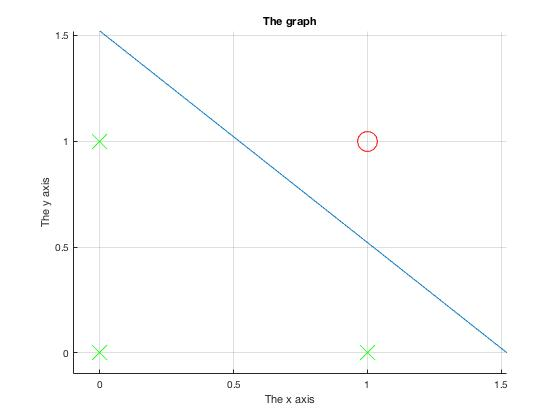
\includegraphics[scale= 0.8]{fig1.jpg}\\
	Result of {\tt hw1conjunction.txt}:

	    $\vec{w^T}$ = $(2.9104,-2.0498,0.1775,190.5196,0.1399,-3.1010,-2.9534,-193.2778,1.1679,-8.8942)$ \\ 
	    $\theta$ = -90.2115 \\ 
	    $\delta$ =-2.4158e-13 $\approx$ 0\\ 
   According to the $\vec{w^T}$, we can infer the conjunction as $x_3 \land \lnot x_7$ because $w_3$ is a large positive coefficient and  $w_7$ is a small negative coefficient. Other $w_i$ are nonzero but relatively small comparing to $\theta$. Even we add all of $|w_i|$ except $w_3$ and $w_7$, the result is not large enough to change our decision. Besides, $\delta$ is almost equal to 0 which is our target of this linear programming problem. All the evidences show that the program works as we expect and can give us a right estimated answer.
\clearpage
\item [(b.3)]
	The result:\\
	$\delta = 1.2619e-09 \approx 0$, accuracyInTrain = 1, accuracyInTest =1\\
	Here, we get $\delta$ is almost equal to 0 which means the linear programming problem was solved well. The accuracies are perfect which means the training data set is not noisy and the classifier we trained is perfect to the test data set.\\
	The figure below shows the weighs we got. We can immediately find that the weighs of vowels at d = 2 are high in yellow and the others are mostly in blue, negative numbers.\\
	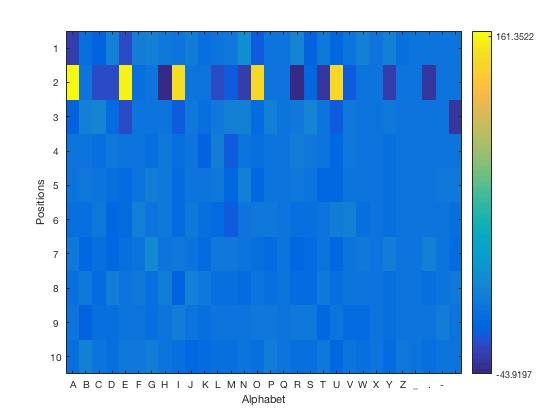
\includegraphics[scale= 0.8]{fig2.jpg}\\ 
	Adjusting {\tt positions = [1 3 4 5]}, we can get a perfect accuracy in the training data set, but an imperfect accuracy in the testing data set (accuracyInTrain = 1, accuracyInTest = 0.8404). Apparently, the figure looks random comparing to original one and there are still some patterns of high weighs which means that the algorithm finds a more complex way to fit our training data and to predict the test data. \\
	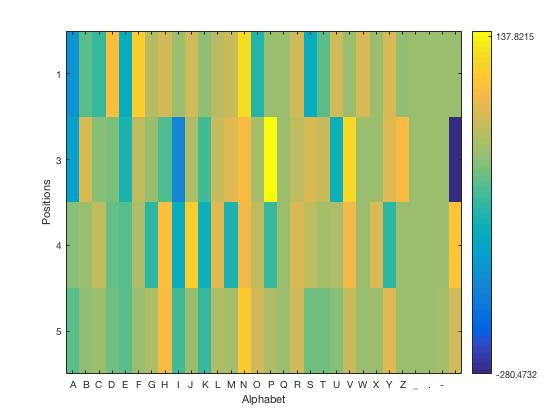
\includegraphics[scale= 0.8]{fig3.jpg}\\ 
	\item [(b.4)]
	There are two ways to achieve $\theta$ finding:\\
	1. Setting a new linear program problem\\
\begin{equation*}
	\vec{c} = \left(\begin{array}{c} 0 \cr 1  \end{array} \right),\ 
	A = \left(\begin{array}{cc} 
	y_1 & 1 &
	y_2 & 1 &
	. & . & 
	. & . & 
	. & . & 
	y_m & 1 &
	0 & 1 
	\end{array} \right),
	\vec{t} = \left(\begin{array}{c} \theta \cr \delta \end{array} \right),\ 
	\vec{b} = \left(\begin{array}{c} 1-y_1\vec{w}^T\vec{x_1} \cr 1-y_2\vec{w}^T\vec{x_2} \cr . \cr . \cr .\cr 1-y_m\vec{w}^T\vec{x_m} \cr 0\end{array} \right)
\end{equation*}\\
2. Giving constraints to Matlab function to make sure $\vec{w}$ will not change.\\
Here, I choose 2 because it is much more faster. Then, we get following figure.\\
\begin{center}
	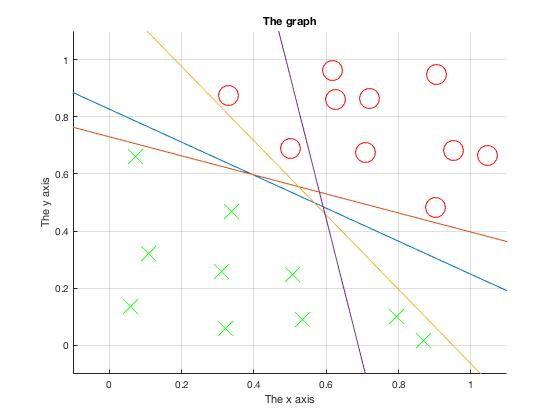
\includegraphics[scale= 0.8]{fig4.jpg}
\end{center}\\
In this script, we fix $\vec{w}$ and find $\theta$ to solve the linear program problem. We get 4 pair of $(\theta,\delta)$, (-243.2630,-1.2506e-12), (-218.9946,-5.1159e-13), (-123.6116,4.2917e-11), (-344.3350,92.9650). First 3 hyperplanes successfully separate the data set and the $\delta$s are close to 0. However, The last hyperplane is apparently failed and the $\delta$ is not close to 0. Although the blue line with more margin between data points in different labels seems the best hyperplane separating the training data set, it is possible that there is an example in the testing data set that blue line cannot separate it right. Also, we can learn from this problem that there are several hyperplanes can separate our training data set. The solution to a linear program problem will not be unique.
\end{itemize}
\clearpage
\item \textbf{Code snippets}\\
{\tt findLinearDiscriminant.m}:\\
\begin{center}
	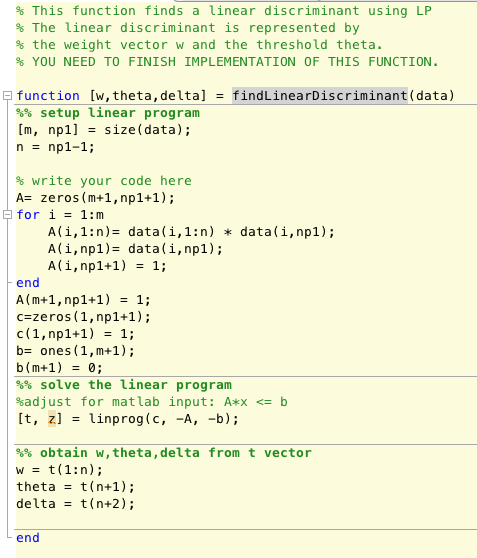
\includegraphics[scale= 0.8]{fig5}
\end{center}b
\clearpage
{\tt computeLabel.m}:\\
\begin{center}
	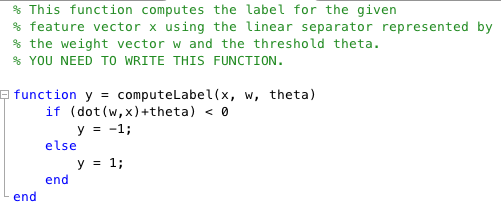
\includegraphics[scale= 0.8]{fig6}
\end{center}
{\tt plot2dSeparator.m}:\\
\begin{center}
	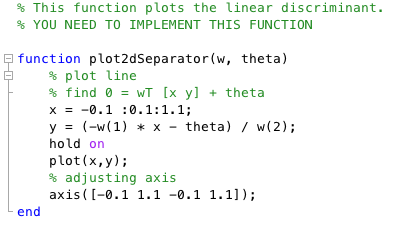
\includegraphics[scale= 0.8]{fig7}
\end{center}
\clearpage
{\tt findLinearThreshold.m}:\\
\begin{center}
	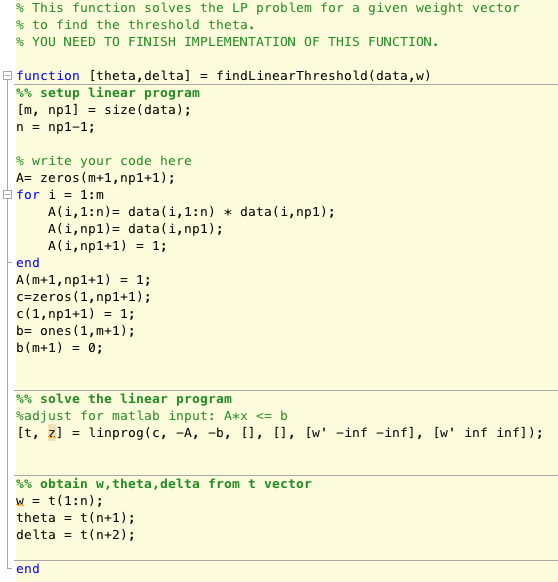
\includegraphics[scale= 0.8]{fig8}
\end{center}

\end{enumerate}

\end{document}